\documentclass[paper=a4paper,fontsize=11pt]{jlreq}
% パッケージの読み込み
\usepackage{luatexja-fontspec}
\usepackage{graphicx}
\usepackage{enumitem} % カスタマイズ用パッケージ
\usepackage{placeins} % 画像のフロートを防止
\usepackage{caption}
\captionsetup[table]{position=top} % すべての表のキャプションを上にする

\setmainfont{Harano Aji Mincho}
\setsansfont{Harano Aji Gothic}
\setmainjfont{Harano Aji Mincho}
\setsansjfont{Harano Aji Gothic}

%句読点置き換え
\usepackage{newunicodechar}
\newunicodechar{、}{,}
\newunicodechar{。}{.}

\usepackage{amsmath,amssymb}
\usepackage{unicode-math}
\setmathfont{LatinModernMath-Regular}

\graphicspath{{img/}}

\makeatletter
% section の番号を part ごとにリセット
\@addtoreset{section}{part}
\makeatother

% partの番号をアラビア数字に変更
\renewcommand{\thepart}{\arabic{part}}
% section の番号を part番号-○○ にする
\renewcommand{\thesection}{\thepart.\arabic{section}}


\title{\huge 令和6年度 修士論文\\\vspace{100truept}プログラム読解における\\視線運動のクラスタリング\\
Clustering of Eye Movements\\ in Program Reading}
\author{\large 大阪公立大学大学院 \\情報学研究科 基幹情報学専攻\\学籍番号 BGA23116\\明石 拓也}


\begin{document}
\maketitle
\clearpage

\tableofcontents
\clearpage

\part{はじめに}
  \section{本研究の背景}
  情報活用能力が必要となった近年において、初等教育からプログラミングが必修化されるなどプログラミング教育の機会は増加している。
  一方で、プログラミングに長けた指導者の不足が問題視されている。そのため、プログラミング学習の支援となるシステムの重要性が高まっている。
  学習システム開発のためには、プログラミングを理解している人の読解方法の傾向をつかむことが重要となっている。\\
  これまで、ソースコード読解時の視線運動を対象とした検証が行われている。被験者にソースコード読解を必要とするタスクを課し、
  読解時の視線運動をアイトラッカーでの計測によりディスプレイ画面上の視線座標という形で取得し、タスクの正誤との関係を調べる分析が主流となっている。
  これまでタスクに利用されてきたソースコードは、変数代入や四則演算のみで構成されるもの、条件分岐や繰り返し文を含むものであるが、
  いずれも単一のクラスを用いた手続き型のソースコードで、数行から十数行程度の短いものである。既存の研究では、クラスオブジェクト生成やポリモーフィズムなど、
  オブジェクト指向の概念を取り入れたソースコードでの検証はなされていない。
  

  \section{本研究の目的}
  本研究は、手続き型ソースコードにおいてプログラミング理解度によって視線運動に差異が発生している現状を踏まえ、
  オブジェクト指向を含むソースコードにおける挙動を明らかにするため行う。
  目的のため、6つのクラスで構成され、オブジェクト生成やメソッド呼び出しを含む百行以上にわたるソースコードを用いて実験を行い、
  クラス単位という従来よりマクロな視点での分析を行う。分析結果の検証のため、被験者ごとの各クラスへの注視時間割合を求め、視線運動の傾向を表すパラメータとする。
  傾向の可視化のため、3次元グラフを用いる。高次元データを3次元グラフで可視化するため、主成分分析で次元圧縮をする。

  \section{本論文の構成}
  本論文では、以下の構成に従って、複数のクラスで構成されるJavaソースコードの読解者の視線運動に対する研究成果の報告を行う。\\
  第2章では本研究に際し提案した手法の紹介をする。\\
  第3章では本研究のため行った実験の準備や手順を説明する。\\
  第4章では実験で得られたデータを加工し、分析する過程とその結果を説明する。\\
  最後に、第5章で本研究のまとめを行う。

\clearpage

\part{提案手法}
  \section{既存の分析手法}
  本研究では、吉岡らが提案した視線移動のマッピング手法\cite{meiji}を流用する。吉岡らは、以下の構成で被験者の視線座標をソースコード中の行・列に変換している。\\
  

  \section{新たに提案する手法}
  本研究で提案する分析手法を以下に示す。
  ・生データから必要な情報を取り出す。
  ・計算によってパラメータを導き出す。
  ・新たなパラメータを分析に使用する。

\clearpage

\part{実験}
  本章では、実験の目的、実験に際し行った準備、当日の手順、得られたデータの概要を示す。\\

  \section{実験の目的}
  本実験は、以下の目的で行う。\\
  ・Javaの基礎知識を有する被験者が、複数のクラスで構成され100行以上にわたる比較的長大なJavaソースコードを読解する際の視線情報の収集。\\
  ・上述のソースコード読解時の被験者のJava理解度の収集\\

  目的達成のため、アイトラッカーを用いて視線情報を収集する。

  実験では、オブジェクト指向の概念を含まない問題2問、含む問題3問の計5つの問題に取り組んでもらった。

  \section{実験対象}
  実験は、近畿大学工業高等専門学校情報科4年生の学生27名を対象とする。被験者全員がオブジェクト指向を含むJavaプログラミングの授業を受講した経験がある。\\
  なお、対象者全員に以下の事項を伝え、承諾書にサインしてもらった。\\
  ・実験で使用する装置が身体に害を及ぼさないこと\\
  ・計測されたデータを個人を特定できないよう十分配慮した上で研究発表に使用すること\\
  ・被験者となるかは任意であり、実験結果が学校の成績等に一切の影響を与えないこと\\
  \\
  
  \section{実験手順}
  実験は、以下の手順で行う。
  \begin{enumerate}
    \item 実験準備
      \begin{enumerate}
        \item iTrace-Atomプラグインの開発
        \item 各PCの環境構築
        \item 実験台のセットアップ
      \end{enumerate}
    \item 実験本番
      \begin{enumerate}
        \item 解答用紙への氏名記入・同意書記入
        \item キャリブレーション
        \item 実験の流れの説明
        \item 練習問題
        \item 5つのタスク提示・視線座標計測
      \end{enumerate}
  \end{enumerate}

  \section{使用するソースコード}
    ソースコードはJavaで記述し、Mainクラスを含む計6つのクラスで構成されるものを準備する。Mainクラス中に5つのタスクにまつわる記述を設けている。\\
    以下に、使用するソースコードの全体像を示す。
    \begin{figure}[h]
      \centering
      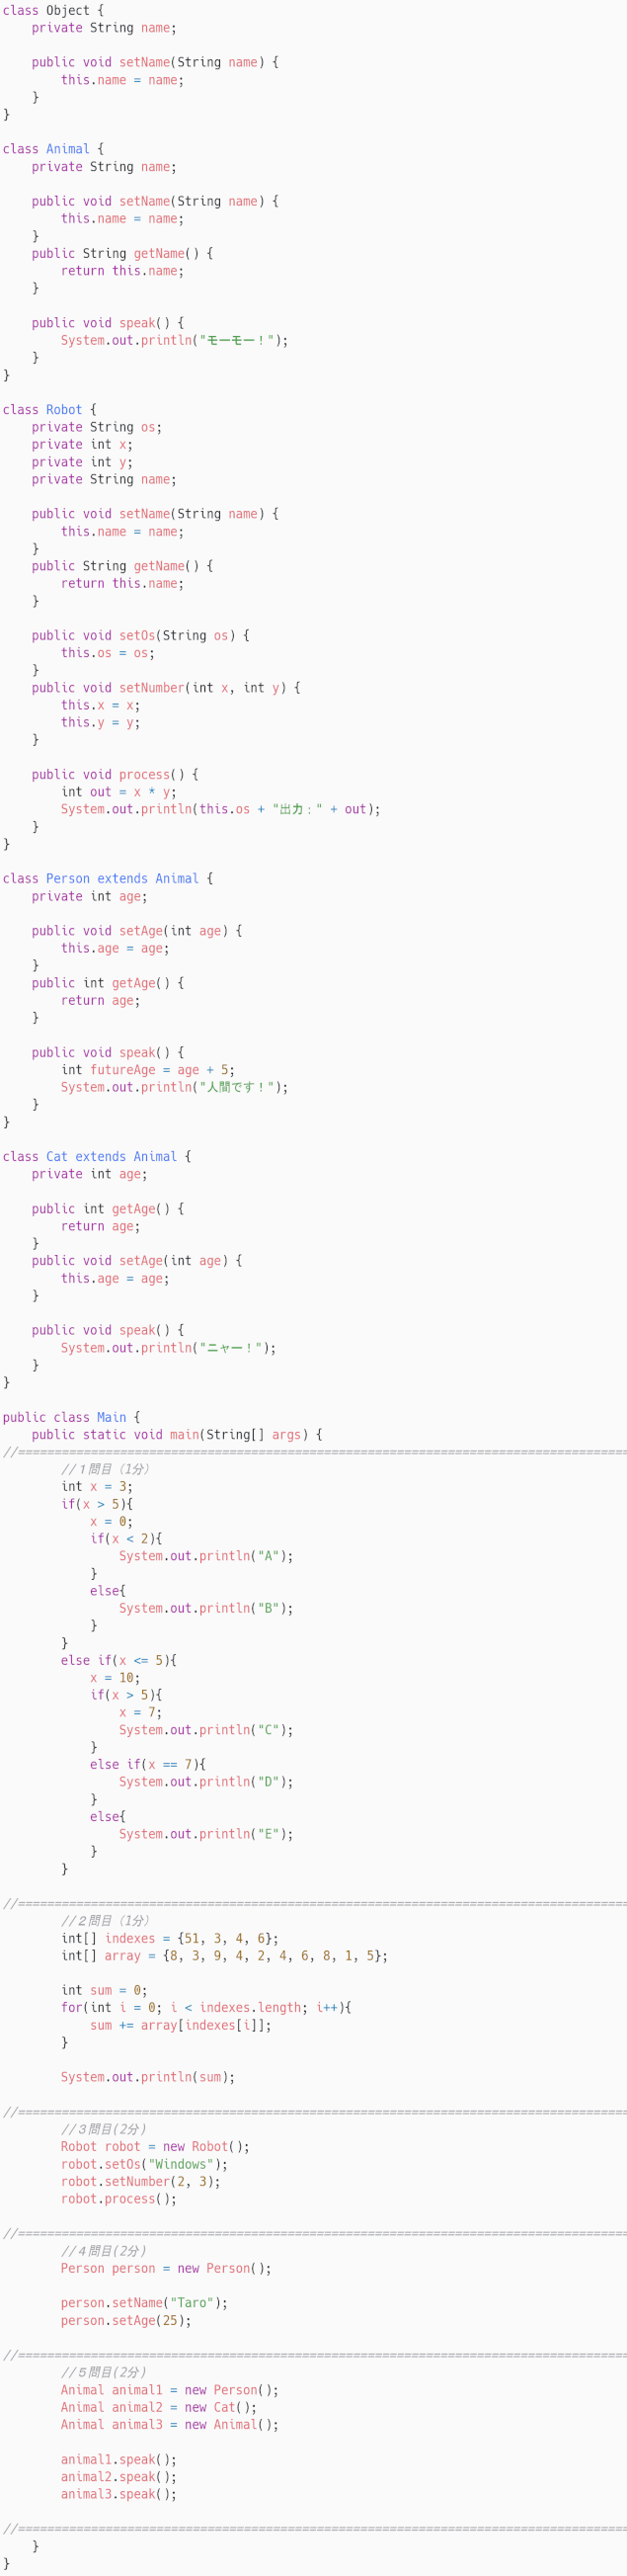
\includegraphics[height=\textheight]{carbon_clip_resized.png}
      \caption{使用したソースコード}
    \end{figure}
    \FloatBarrier

  \section{被験者に課すタスク}
    タスクは全5問用意する。うち2問がオブジェクト指向の概念を伴わないMainクラス内で完結するタスク、うち3問がオブジェクト指向の概念を伴うタスクである。
    以下にタスクの内容を示す。\\
    \begin{enumerate}[label=タスク\arabic*:]
      \item 変数代入とif文による条件分岐を組み合わせたタスク。標準出力の出力結果を答えさせる。
      \begin{figure}[h]
        \centering
        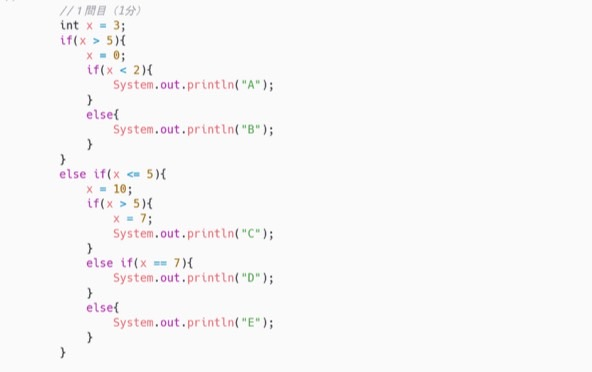
\includegraphics[height=0.5\linewidth]{プログラム画像_タスク1.jpg}
        \caption{タスク1のソースコード}
      \end{figure}
      \FloatBarrier
      \item 配列の参照を使用したタスク。標準出力の出力結果を答えさせる。
      \begin{figure}[h]
        \centering
        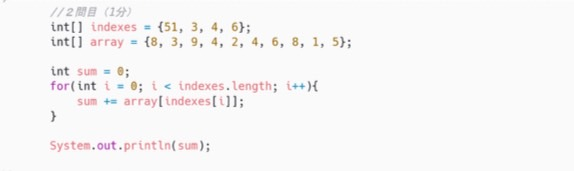
\includegraphics[height=0.25\linewidth]{プログラム画像_タスク2.jpg}
        \caption{タスク2のソースコード}
      \end{figure}
      \FloatBarrier
      \item 1種類のクラスを使用し、オブジェクト生成と外部からのメソッド実行を含むタスク。標準出力の出力結果を答えさせる。
      \begin{figure}[h]
        \centering
        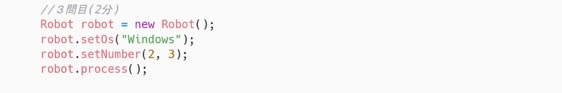
\includegraphics[height=0.2\linewidth]{プログラム画像_タスク3.jpg}
        \caption{タスク3のソースコード}
      \end{figure}
      \FloatBarrier
      \item 2種類のクラスを使用し、オブジェクト生成とゲッター・セッターの呼び出しを含むタスク。2種類のクラスは片方がもう片方を継承する関係にある。ソースコード内で、それぞれのオブジェクトのセッターが定義された行を答えさせる。
      \begin{figure}[h]
        \centering
        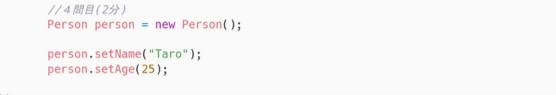
\includegraphics[height=0.2\linewidth]{プログラム画像_タスク4.jpg}
        \caption{タスク4のソースコード}
      \end{figure}
      \FloatBarrier
      \item 3種類のクラスを使用し、メソッドのオーバーライドを含む。標準出力の出力結果を答えさせる。
      \begin{figure}[h]
        \centering
        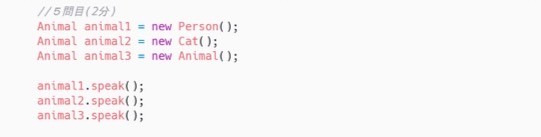
\includegraphics[height=0.25\linewidth]{プログラム画像_タスク5.jpg}
        \caption{タスク5のソースコード}
      \end{figure}
      \FloatBarrier
    \end{enumerate}

  

  \section{実験に使用する物品}
    実験に際して、以下の物が必要となる。
    \begin{enumerate}
      \item アイトラッカー
      \item アイトラッカーの設定・キャリブレーションに用いるソフトウェア(Tobii Pro Eye Tracker Manager)
      \item アイトラッカーの処理を担当するソフトウェア(iTrace Core)
      \item タスクに使用するソースコードを表示するエディタ(Atom)
      \item アイトラッカーで取得した画面上での座標を、ソースコードの行・列に変換する為のプラグイン
    \end{enumerate}
    以下、これらの物を解説する。

    \subsection{アイトラッカー}
      視線運動をディスプレイ画面上の時系列座標データとして取得するため,アイトラッカーと呼ばれる装置を使用する.本研究では,3台のディスプレイで同時に測定するため、計3台のアイトラッカーを準備する。
      内訳として、Tobii Pro Spark\cite{spark}2台とTobii Pro Nano\cite{nano}1台を使用する。
      \\
      Tobii Pro Spark、Tobii Pro Nanoともにディスプレイ装置の下部に固定することで,ディスプレイ画面上における被験者の注視点の座標を計測できる.
      サンプリングレートはいずれも60Hzである.測定の際,各被験者ごとにキャリブレーションする.

    \subsection{Tobii Pro Eye Tracker Manager}
      アイトラッカーのパラメータ設定、キャリブレーションにはTobii公式で提供されているTobii Pro Eye Tracker Managerというソフトウェアを使用する。
    
    \subsection{アイトラッカーの処理を担当するソフトウェア}
      アイトラッカーの測定開始・終了処理や、出力データの成型などを担当するソフトウェアとしてiTrace Core\cite{itrace}を使用する。

    \subsection{タスクに使用するソースコードを表示するエディタ(Atom)}
      エディタは、iTraceプラグインとの互換性のため、Atom\cite{atom}を使用する。

    \subsection{iTrace-Atomプラグイン}
      iTraceの出力座標データとエディタの画面表示情報を結びつけ、座標からプログラム中の行・列に対応させるため、Atomエディタのプラグインが開発されている。\\
      本研究では、Github上で公開されているiTrace-Atomプラグインに機能を追加したものを用いる。
    
      
    \subsection{ディスプレイ}
      画面サイズ1920×1200ピクセルのモニタを使用する。

    \subsection{コンピュータ}
      Windows11がセットアップされたコンピュータを使用する。
  
  \section{実験準備}
    実験で使用する


  \section{実験}
    本章では、実験の流れを示す。本実験により、データは問1~問5で27人分得られた。

    近畿大学工業高等専門学校情報科4年生の学生27名を対象として行う。対象者全員がオブジェクト指向を含むJavaプログラミングの授業を受講した経験がある。\\
    実験では、オブジェクト指向の概念を含まない問題2問、含む問題3問の計5つの問題に取り組んでもらった。なお、対象者全員に計測するデータを研究以外の用途
    に使用しない旨を伝え、承諾書にサインしてもらった。
    3台の実験台を用い、3人ずつ同時並行で測定する。実験の流れを以下に示す。\\
    
    承諾書にサインしてもらう
    解答用紙に、出席番号と名前を書いてもらう
    3台の実験台それぞれに座ってもらい、キャリブレーションを行う。
    実験の流れの説明。
    ソースコードを読んで問題を解くこと、その際の視線データを計測すること、
    スクロール操作のみ行い、コードへの書き込みを行わないこと、回答がわかり次第挙手で合図し、解答用紙に書き込むこと、


    \begin{figure}[htbp]
      \centering
      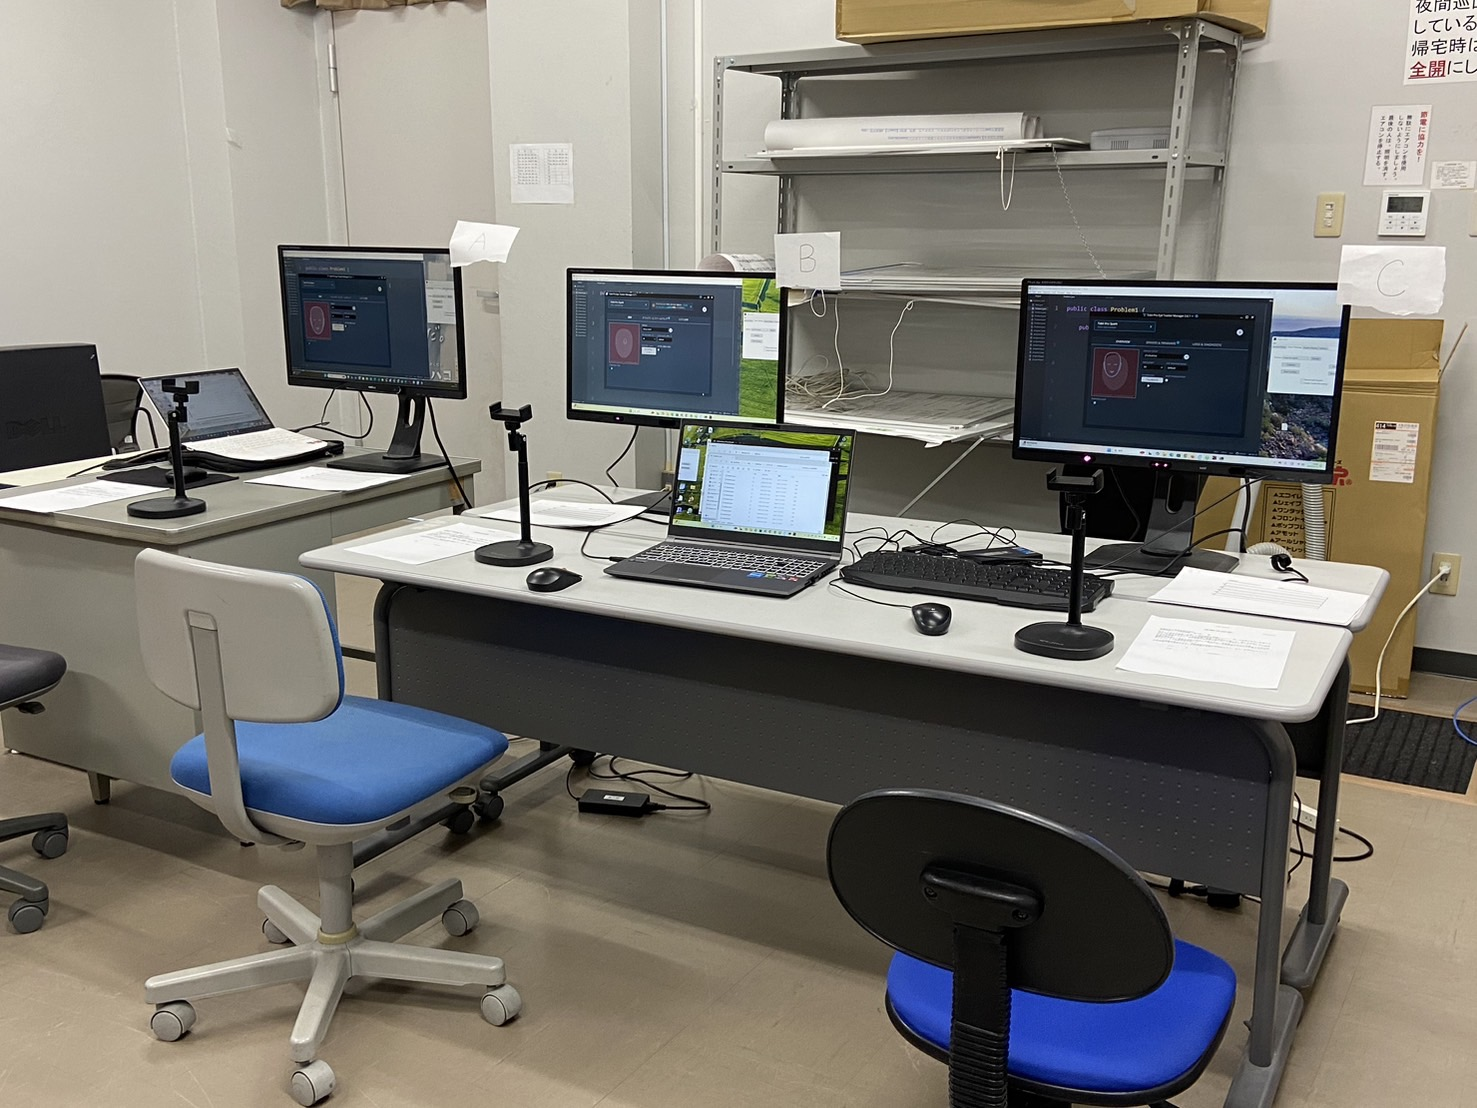
\includegraphics[width=0.8\linewidth]{実験部屋.jpg}
      \caption{実験部屋の様子}
    \end{figure}
    \FloatBarrier
  
  \section{実験結果}
    実験により、\\
    なお、各被験者のタスクへの正誤は以下の通りとなった。\\


\clearpage

\part{データの分析}
  本章では、実験で得られたデータを加工し、分析する一連の流れを示す。

  \section{はじめに}
   実験により得られた生データはxml形式で保存される。以下に、生データが持つパラメータを記す。\\
    \begin{table}[h]
      \centering
      \caption{生データに含まれるデータ一覧}
      \begin{tabular}{|c|c|c|}
        \hline
        パラメータ名 & 値の意味 & 値の例 \\ \hline
        screen\_width & ディスプレイ画面の横px数 & 1920 \\ \hline
        screen\_height & ディスプレイ画面の縦px数 & 1200 \\ \hline
        plugin\_type & プラグインの種類 & ATOM \\ \hline
        gaze & 視線情報 & 後述 \\ \hline
      \end{tabular}
      \label{tab:basic}
    \end{table}
   \FloatBarrier

   gazeパラメータはアイトラッカーのサンプリング数だけ存在し、それぞれ以下のパラメータを持つ。

  \begin{table}[h]
    \centering
    \caption{生データに含まれる視線情報}
    \begin{tabular}{|c|c|c|}
        \hline
        パラメータ名 & 値の意味 & 値の例 \\ \hline
        event\_id & 2 & 133784518694431017 \\ \hline
        plugin\_time & サンプリングのUNIX時間[ms] & 1733978269442 \\ \hline
        x & ディスプレイ画面上のx座標[px] & 480 \\ \hline
        y & ディスプレイ画面上のy座標[px] & 418 \\ \hline
        source\_file\_line & ソースコード中の行 & 2 \\ \hline
        source\_file\_col & ソースコード中の列 & 9 \\ \hline
        word & 視線が位置していた単語 & int \\ \hline
        gaze\_target & 視線が位置していたファイルの名前 & Problem1.java \\ \hline
        gaze\_target\_type & 対象ファイルの拡張子 & java \\ \hline
        source\_file\_path & 対象ファイルのファイルパス & Problem1.java \\ \hline
        editor\_line\_height & エディタの行の高さの設定値 & 40 \\ \hline
        editor\_font\_height & エディタのフォントサイズの設定値 & 120 \\ \hline
    \end{tabular}
    \label{tab:basic}
  \end{table}
  \FloatBarrier
  
  上述の生データから特定の情報を抜き出し、プログラムで扱いやすいようcsvに加工する。
  csvから、クラスごとの注視時間割合を算出
  注視時間割合を主成分分析で3次元まで落とし、正誤で色分けして3Dプロットで可視化
  可視化したデータを観察する。
  
  \section{3Dプロットの観察}
    \begin{figure}[htbp]
      \centering
      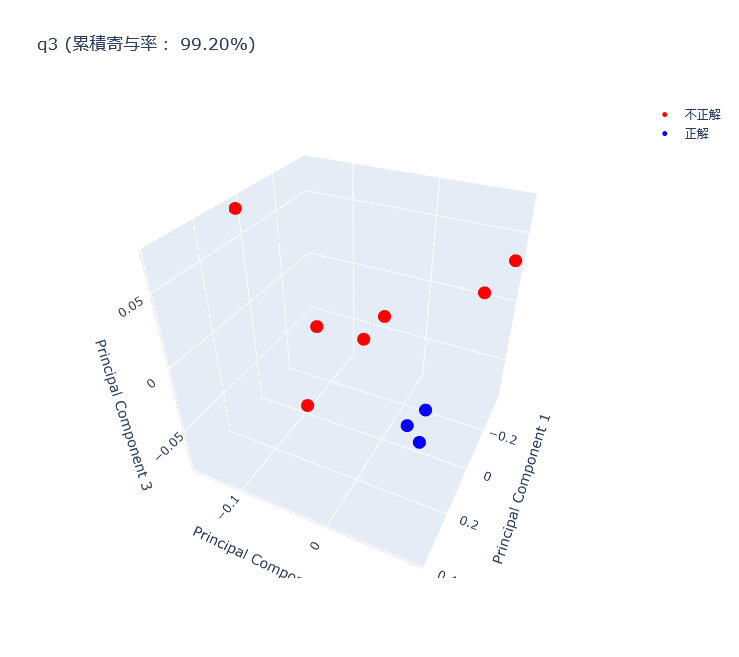
\includegraphics[width=0.8\linewidth]{3dplot_q3.png}
      \caption{タスク3の分布}
    \end{figure}
    \FloatBarrier
    \begin{figure}[htbp]
      \centering
      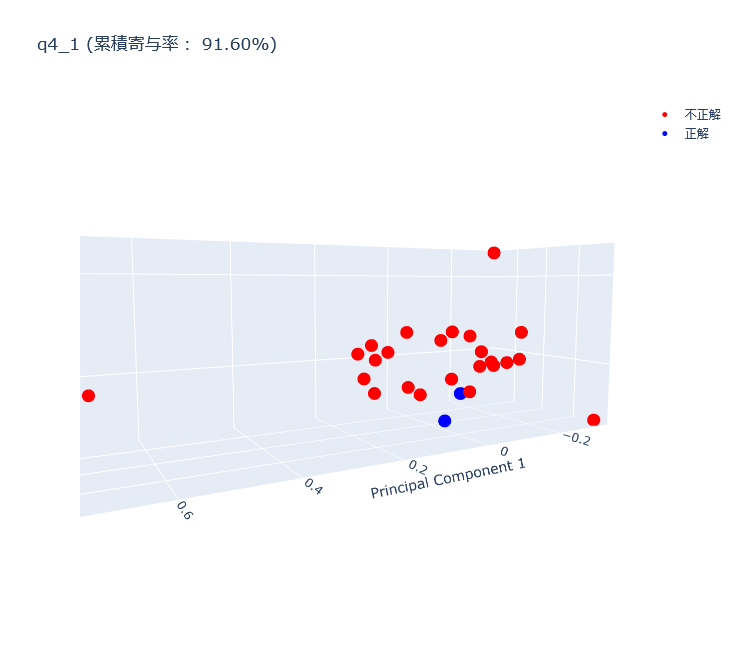
\includegraphics[width=0.8\linewidth]{3dplot_q4_1.png}
      \caption{タスク4-1の分布}
    \end{figure}
    \FloatBarrier
    \begin{figure}[htbp]
      \centering
      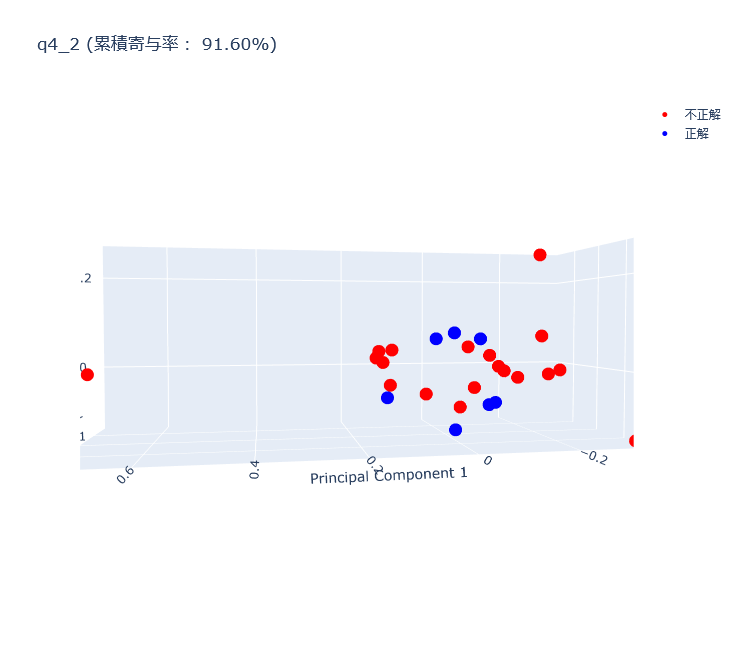
\includegraphics[width=0.8\linewidth]{3dplot_q4_2.png}
      \caption{タスク4-2の分布}
    \end{figure}
    \FloatBarrier
    \begin{figure}[htbp]
      \centering
      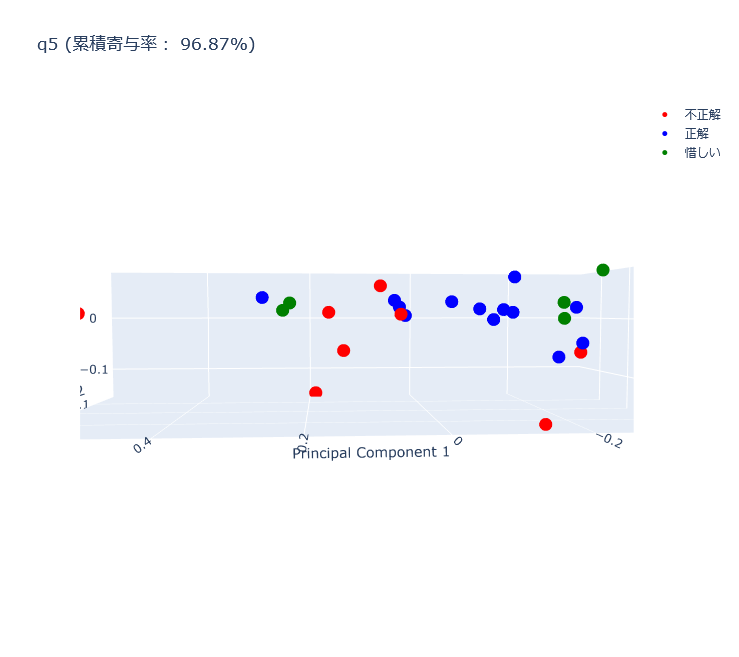
\includegraphics[width=0.8\linewidth]{3dplot_q5.png}
      \caption{タスク5の分布}
    \end{figure}
    \FloatBarrier

    いずれのタスクにおいても、正解者と不正解者で異なる分布になっていることが分かる。

\clearpage    

\part{結論}
本研究により、オブジェクト指向を取り入れたタスクにおいて、正答者の視線運動は3次元グラフ上のある一定の範囲に固まる傾向があり、
不正答者のものはよりばらつきが大きいことが分かった。主成分分析での次元圧縮の際に算出した累積寄与率は90%以上と高く、
圧縮前のパラメータでもおおむね同様の傾向であるといえる。このことから、オブジェクト指向を取り入れたソースコードを用いたタスクを課すことにより、
読解者がコードを理解していない可能性を検知できることが示唆された。

\pagebreak

\part{謝辞}
本研究は,
大阪公立大学情報学研究科・情報処理領域の大野修一先生,
所属の岩佐英彦先生,
近畿大学工業高等専門学校情報科5年生の岡村晏志様、
および視線情報測定に協力して頂いた近畿大学工業高等専門学校・情報科4年生27名の協力により得られた成果である.ここに記して謝意を表します.

\pagebreak

\begin{thebibliography}{99}
  \bibitem{meiji} 視線分析の傾向分析による特徴抽出
  \bibitem{uwano} 構文木と視線移動の自動マッピング手法を用いたプログラム理解過程の分析,吉岡春彦,上野秀剛,2023
  \bibitem{spark} tobii pro spark https://www.tobii.com/ja/products/eye-trackers/screen-based/tobii-pro-spark
  \bibitem{manager} Tobii Pro Eye Tracker Manager https://connect.tobii.com/s/etm-download
  \bibitem{nano} https://www.tobii.com/ja/products/discontinued/tobii-pro-nano
  \bibitem{itrace} iTrace https://www.i-trace.org/
  \bibitem{atom} ATOM https://atom-editor.cc/
\end{thebibliography}


\end{document}
